% fig1-triangle.tex --- Figure 1 of the Letter: the lattice infrared triangle.
%
% Standalone; compile with:  pdflatex fig1-triangle.tex
% Target: PRL single column, 8.6 cm wide.
%
% Every status label in this figure is copied from claims/CLAIMS.md as of
% 2026-08-29.  Do not change a status here without changing the DAG row.
% Draft caption at the end of this file.
%
\documentclass[border=1pt]{standalone}
\usepackage[T1]{fontenc}
\usepackage{newtxtext,newtxmath}   % Times, to match revtex4-2/aps
\usepackage{amsmath}               % amssymb clashes with newtxmath (\Bbbk)
\usepackage{xcolor}
\usepackage{tikz}
\usetikzlibrary{arrows.meta,calc}

% --- black plus two muted accents ----------------------------------------
\definecolor{cprv}{RGB}{28,74,112}    % PROVED
\definecolor{cskt}{RGB}{158,94,30}    % SKETCH / REFUTED

% --- print sizes, chosen for legibility at 8.6 cm -------------------------
\newcommand{\ttl}{\fontsize{7.6}{8.8}\selectfont\bfseries}
\newcommand{\bdy}{\fontsize{6.6}{8.0}\selectfont}
\newcommand{\sml}{\fontsize{5.7}{6.9}\selectfont}

\newcommand{\stprv}{{\color{cprv}\bfseries PROVED}}
\newcommand{\stskt}{{\color{cskt}\bfseries SKETCH}}
\newcommand{\stref}{{\color{cskt}\bfseries REFUTED}}
\newcommand{\ids}[1]{{\color{black!55}\itshape #1}}
\newcommand{\gap}[1]{{\color{cskt}#1}}

\begin{document}
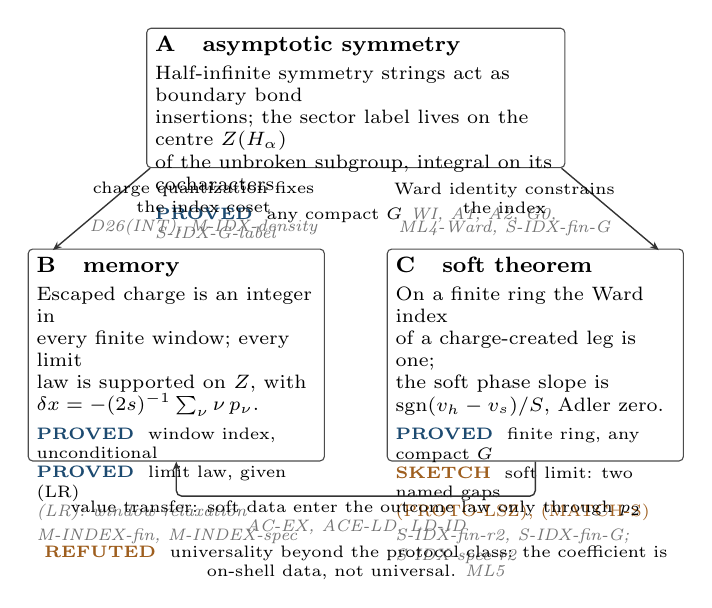
\begin{tikzpicture}[
  cbox/.style={draw=black!70, line width=0.4pt, rounded corners=1.6pt,
               inner sep=3pt, fill=white},
  flow/.style={draw=black!80, line width=0.5pt,
               -{Stealth[length=3.2pt,width=2.6pt]}},
  elab/.style={align=center, inner sep=1pt, font=\sml},
]

% ============================ corner A ====================================
\node[cbox, anchor=south] (A) at (0,1.02) {%
  \parbox[t][1.56cm][t]{5.10cm}{%
    \raggedright
    {\ttl A\quad asymptotic symmetry\par}%
    \vspace{2pt}%
    {\bdy
      Half-infinite symmetry strings act as boundary bond\\
      insertions; the sector label lives on the centre $Z(H_\alpha)$\\
      of the unbroken subgroup, integral on its cocharacters.\par}%
    \vspace{3.5pt}%
    {\sml \stprv{} \ any compact $G$
      \hfill \ids{WI, A1, A2, G0, S-IDX-G-label}\par}%
  }};

% ============================ corner B ====================================
\node[cbox, anchor=north] (B) at (-2.28,0) {%
  \parbox[t][2.48cm][t]{3.55cm}{%
    \raggedright
    {\ttl B\quad memory\par}%
    \vspace{2pt}%
    {\bdy
      Escaped charge is an integer in\\
      every finite window; every limit\\
      law is supported on $\mathbb{Z}$, with\\
      $\delta x=-(2s)^{-1}\sum_\nu \nu\,p_\nu$.\par}%
    \vspace{3.5pt}%
    {\sml
      \stprv{} \ window index, unconditional\\
      \stprv{} \ limit law, given (LR)\\
      \ids{(LR): window relaxation}\\[2pt]
      \ids{M-INDEX-fin, M-INDEX-spec}\par}%
  }};

% ============================ corner C ====================================
\node[cbox, anchor=north] (C) at (2.28,0) {%
  \parbox[t][2.48cm][t]{3.55cm}{%
    \raggedright
    {\ttl C\quad soft theorem\par}%
    \vspace{2pt}%
    {\bdy
      On a finite ring the Ward index\\
      of a charge-created leg is one;\\
      the soft phase slope is\\
      $\operatorname{sgn}(v_h-v_s)/S$, Adler zero.\par}%
    \vspace{3.5pt}%
    {\sml
      \stprv{} \ finite ring, any compact $G$\\
      \stskt{} \ soft limit: two named gaps\\
      \gap{(PROTO-LSZ), (MATCH-S)}\\[2pt]
      \ids{S-IDX-fin-r2, S-IDX-fin-G; S-IDX-spec-r2}\par}%
  }};

% ============================ edges =======================================
% A ==> B
\draw[flow] ($(A.south west)+(0.05,0)$) -- ($(B.north west)+(0.32,-0.02)$);
\node[elab, anchor=east, inner sep=0pt] at (-0.48,0.50) {%
  charge quantization fixes\\ the index coset\\
  \ids{D26(INT), M-IDX-density}};

% A ==> C
\draw[flow] ($(A.south east)+(-0.05,0)$) -- ($(C.north east)+(-0.32,-0.02)$);
\node[elab, anchor=west, inner sep=0pt] at (0.48,0.50) {%
  Ward identity constrains\\ the index\\
  \ids{ML4-Ward, S-IDX-fin-G}};

% C ==> B  (routed below the base so the label gets the full width)
\coordinate (bl) at ($(B.south)+(0,-0.44)$);
\coordinate (br) at ($(C.south)+(0,-0.44)$);
\draw[flow, rounded corners=2pt] (C.south) -- (br) -- (bl) -- (B.south);
\coordinate (mid) at ($(bl)!0.5!(br)$);
\node[elab, anchor=north, inner sep=0pt] at ($(mid)+(0,-0.05)$) {%
  value transfer: soft data enter the outcome law only through $p_2$\\
  \ids{AC-EX, ACE-LD, LD-ID}};

% ============================ the fourth result ===========================
\node[anchor=north, inner sep=0pt] at ($(mid)+(0,-0.62)$) {%
  \parbox{8.32cm}{\centering\sml
    \stref{} \ universality beyond the protocol class: the coefficient is
    on-shell data, not universal. \ids{ML5}\par}};

\end{tikzpicture}
\end{document}

% =========================================================================
% DRAFT CAPTION (to be moved into \caption{} in main.tex when Fig. 1 lands)
% =========================================================================
%
% \caption{The infrared triangle of a quantum spin chain, annotated with the
%   status each corner has reached here.  Symmetry quantizes the infrared
%   data; the excitation ansatz supplies the kinematics; dynamics only picks
%   the values.  (A)~Asymptotic symmetry is proved for any compact on-site
%   group $G$: half-infinite symmetry strings act as boundary bond
%   insertions, and the sector label lives on the centre of the unbroken
%   subgroup, where it is integral on cocharacters.  (B)~Memory is proved
%   with no scattering input.  The escaped charge of a finite window is an
%   integer unconditionally, and every subsequential outcome law of the
%   two-point measurement protocol is supported on $\mathbb{Z}$ with
%   $\delta x=-(2s)^{-1}\sum_\nu \nu p_\nu$, conditionally on the
%   window-relaxation hypothesis~(LR).  (C)~The soft theorem is proved on a
%   finite ring, where the Ward identity forces the index of a
%   charge-created leg to be exactly one, at $SU(2)$ and at any compact $G$;
%   the soft limit itself is so far a sketch, with two named gaps -- an LSZ
%   reduction for the protocol datum, (PROTO-LSZ), and the on-shell matching
%   that identifies the fixed-time readout with the multiplier, (MATCH-S).
%   The edges carry the implications we actually establish: charge
%   quantization fixes the coset on which the memory index lives, the Ward
%   identity constrains that index, and soft data reach the outcome law only
%   through the single weight $p_2$.  Universality of the soft factor beyond
%   the protocol class is refuted, which is why the coefficient in (C) is
%   on-shell data rather than a universal number.  Small italic labels are
%   identifiers in the claim DAG.}
%
% Identifiers in full, by corner:
%   A     : WI, A1, A2, G0 (Corner A, converged r3); S-IDX-G-label;
%           M-IDX-density
%   B     : M-INDEX-fin (unconditional), M-INDEX-spec (conditional on
%           D27(LR1--LR3))
%   C     : S-IDX-fin-r2, S-IDX-fin-G (PROVED); S-IDX-spec-struct-r2 and
%           S-IDX-spec-r2 (SKETCH; gaps (PROTO-LSZ), (MATCH-S))
%   edges : D26(INT), M-IDX-density | ML4-Ward, S-IDX-fin-G |
%           AC-EX, ACE-LD (ACE-LD-eps, ACE-LD-sharp), LD-ID
%   fourth result : ML5 (REFUTED); M / Conjecture-M (REFUTED)
